% =====================================================================
%  PHẦN: CÁC CHỨC NĂNG CHÍNH CỦA GAME TETRIS
%  Người viết: Võ Ngọc Thơ
% =====================================================================

Dựa trên quy chuẩn thiết kế trò chơi Tetris hiện đại (\textit{Tetris Guideline}) và định hướng phát triển sản phẩm của nhóm, các chức năng chính của game Tetris được xây dựng bao gồm các nhóm cơ chế cốt lõi sau~\cite{tetris_guideline}:

\subsection{Cơ chế sinh và quản lý khối gạch (Tetromino Management)}
\begin{itemize}
    \item \textbf{Tạo khối ngẫu nhiên chuẩn 7-bag:} Trò chơi sử dụng thuật toán xáo trộn nhóm 7 khối gạch tiêu chuẩn ($I, J, L, O, S, T, Z$). Cơ chế này đảm bảo người chơi nhận đủ cả 7 loại khối trong mỗi chu kỳ 7 lượt, hạn chế tình trạng xuất hiện trùng lặp quá nhiều hoặc thiếu khối cần thiết~\cite{tetris_randomizer}.
    \item \textbf{Khởi tạo khối (Spawn Location):} Khối gạch mới xuất hiện ở chính giữa phía trên đỉnh của lưới chơi trước khi tự động rơi xuống.
\end{itemize}

\begin{figure}[H]
    \centering
    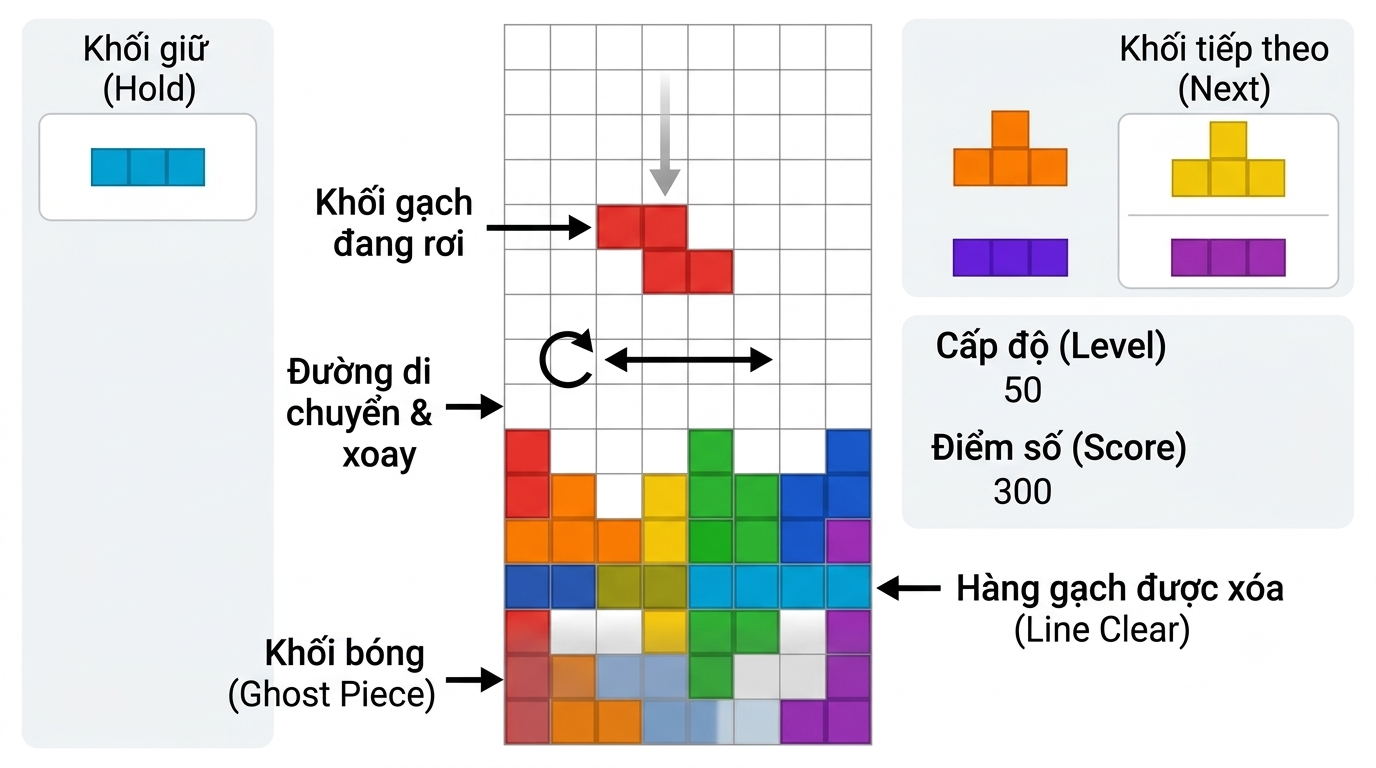
\includegraphics[width=0.75\textwidth]{imgs/chuc_nang_game.png}
    \caption{Sơ đồ minh họa các chức năng và cơ chế hoạt động chính của game Tetris}
    \label{fig:cac_chuc_nang}
\end{figure}

\subsection{Hệ thống tương tác và điều khiển khối (Block Manipulation)}
\begin{itemize}
    \item \textbf{Di chuyển ngang:} Cho phép dịch chuyển khối sang trái hoặc phải theo từng ô vuông hoặc di chuyển liên tục khi giữ phím.
    \item \textbf{Xoay khối (Super Rotation System - SRS):} Cho phép xoay khối $90^\circ$ theo chiều kim đồng hồ hoặc ngược chiều kim đồng hồ, tích hợp cơ chế xử lý va chạm (\textit{Wall Kick}) giúp khối xoay linh hoạt ngay cả khi sát tường~\cite{tetris_guideline}.
    \item \textbf{Rơi chậm (Soft Drop) và Rơi nhanh (Hard Drop):} 
    \begin{itemize}
        \item \textit{Soft Drop:} Tăng tốc độ rơi của khối gạch trong khi người chơi giữ phím điều hướng xuống.
        \item \textit{Hard Drop:} Thả khối gạch rơi lập tức xuống vị trí thấp nhất và khóa cố định tại đó.
    \end{itemize}
    \item \textbf{Thời gian trễ khóa (Lock Delay):} Cung cấp một khoảng thời gian ngắn sau khi khối tiếp đất để người chơi tiếp tục điều chỉnh vị trí trước khi khối bị khóa hẳn~\cite{tetris_lock}.
\end{itemize}

\subsection{Các chức năng giao diện hỗ trợ người chơi (UI/UX)}
Như được minh họa ở Hình~\ref{fig:cac_chuc_nang}, giao diện trò chơi cung cấp các tính năng bổ trợ quan trọng:
\begin{itemize}
    \item \textbf{Xem trước khối tiếp theo (Next Piece Preview):} Hiển thị khối gạch sắp xuất hiện ở bảng phụ bên cạnh, giúp người chơi chủ động tính toán chiến thuật.
    \item \textbf{Cất giữ khối (Hold Piece):} Cho phép tạm lưu khối gạch hiện tại vào ô dự trữ và đổi lấy khối khác khi cần. Mỗi khối mới chỉ được thực hiện thao tác cất giữ tối đa 1 lần.
    \item \textbf{Khối bóng gợi ý (Ghost Piece):} Hiển thị bóng mờ của khối gạch ở đáy lưới, giúp xác định chính xác vị trí khối sẽ đáp xuống.
\end{itemize}

\subsection{Xử lý xóa hàng, tính điểm và tăng cấp độ}
\begin{itemize}
    \item \textbf{Xóa hàng và Tính điểm:} Khi một hàng ngang được lấp đầy 10 ô gạch, hàng đó sẽ tự động biến mất và các khối phía trên dời xuống. Hệ thống thưởng điểm cao hơn khi xóa nhiều hàng cùng lúc (Single, Double, Triple, Tetris) hoặc thực hiện các chuỗi xóa liên tiếp (\textit{Combo}, \textit{Back-to-Back})~\cite{tetris_scoring}.
    \item \textbf{Tăng cấp độ (Level Progression):} Tốc độ rơi của khối tăng dần theo cấp độ (hoặc sau mỗi 10 hàng xóa được), tạo ra độ khó và áp lực thời gian tăng dần~\cite{tetris_marathon}.
    \item \textbf{Kết thúc trò chơi (Game Over / Top Out):} Trò chơi dừng lại và thông báo kết thúc khi khối gạch mới bị chồng lấn hoặc không thể xuất hiện thêm trong vùng chơi~\cite{tetris_topout}.
\end{itemize}
